
\chapter{Existing Literature}
\label{Chap:Lit}

\section{Introduction to Lighting}
\label{sec:LitIntro}

Many people do not realise how much time they spend in un-natural lighting conditions. In 2001, a study published in \textit{Nature} magazine found that the average American spends more than three quarters of their time inside \citep{klepeisNationalHumanActivity2001}. More recent studies have put this number as high as 90\% \citep{opiniumBritsSpend902018}, and when most buildings do not get adequate sunlight in the day, the time spent under man-made light sources can be significant. Furthermore, after dark, almost all buildings are lit artificially, very few people around the world do not spend their nights in lit environments.

\citet{falchiNewWorldAtlas2016} found that 86\% of the worlds population, and 99\% of the US and European population live under ``light polluted'' skies. The world uses so much light, that one third of humanity, 60\% of Europeans, and 80\% of North Americans cannot see the Milky Way. These statistics highlight just how pervasive artificial light is in the modern age.


\section{Lighting Technologies}

\subsection{How did we get here?}

It wasn't always this way. For only the most recent 1.5 million years - a blink of the evolutionary eye - have humans been able to harness the power of fire to extend the usable time of day \citep{gowlettEarliestFireAfrica2013}. It is important to note, however, that fire does not try to emulate daylight: fires used after dark were used for cooking and as a social space \citep{gowlettDiscoveryFireHumans2016}.

It was not until Humphrey Davy and Michael Faraday's contributions to science allowed Davy to produce the first functional electric light, the arc lamp \citep{knightHumphryDavyScience1998}. Since that fateful day, humans' relationship with night has grown increasingly distant. In 1878, Swan presented the first  incandescent lamp, patented by Edison in 1880 (though it is believed that others were developing this technology concurrently) \citep{montoyaIndoorLightingTechniques2017a}. These bulbs are very inefficient; the peak wavelength is determined by the temperature of the gas in the bulb. In order for visible emission to occur, very high temperatures must be achieved - and still the majority of the light will be infra-red (IR) and not visible to the human eye \citep{montoyaIndoorLightingTechniques2017a}.

The next widely adopted innovation was discharge lamps such as sodium lamps and fluorescent tubes, as many Correlated Colour Temperatures (CCTs) could be achieved. Compact Fluorescent Tubes (CFTs) could directly replace Incandescent bulbs using the same fittings.

While LEDs gained widespread popularity in the early $21^{st}$ century \citep{matsumotoMeasuringHouseholdAbility2020}, the first visible light LED was produced back in 1962 by Nick Holonyak \citep{holonyakCOHERENTVISIBLELIGHT1962}, based on the even earlier LEDs of Oleg Losev from 1927 \citep{zheludevLifeTimesLED2007}. It wasn't until 1995 that a non-red LED was produced, solving the issue of monochromasity of LED technology (it was blue) \citep{nakamuraInGaNAlGaNBlue1995}.

Once white LEDs could be produced, it led to the ``Third Revolution'' of indoor lighting \citep{montoyaIndoorLightingTechniques2017a}, and now LEDs are ubiquitous in modern life. New LED technology continues to be developed, such as the Organic LED (OLED), which are cheaper and offer better colour rendition. OLED technology has only recently been applied to indoor lighting \citep{phelanOLEDLightingHits2018}, although there are some promising developments in the field \citep{benderSolidStateLightingConcise2015}. However there is still some way to go before OLEDs replace LEDs in artificial lighting technology.

\subsection{Energy Consumption and Environmental Considerations}
\label{sec:Energy}

Incandescent bulbs are not efficient. in fact, they're banned from being sold in the EU because they're so inefficient \citep{Directive201227}. However, this doesn't mean they're all bad, they actually have many benefits; firstly, they are not hazardous, unlike fluorescents and LEDs, which also require higher resource depletion to create \citep{PotentialEnvironmentalImpacts}. But LEDs use 85\% less energy and last 50 times longer than incandescents \citep{mottierLEDLightingApplications2010}. This is significant when considering that 20-40\% of most buildings power consumption is from lighting alone \citep{perez-lombardReviewBuildingsEnergy2008}, accounting for as much as 10\% of all power consumed in Europe \citep{bertoldiEnergyEfficiencyStatus2012}. Considering  this, and that LEDs can theoretically convert 100\% of electrical energy to visable light (thermal regulation is key) \citep{jordanChallengesLEDPackaging2012}, it is clear why the wide scale adoption of LED technology has been so rapid \citep{matsumotoMeasuringHouseholdAbility2020}.



\section{Circadian Rhythms}
\label{sec:Circadian}

\subsection{What is the Circadian Rhythm?}

In 1729, the French scientissst Jean-Jacques d'Ortous de Mairan	used plants kept completely in the dark to determine that their diurnal cycles were not caused by external light stimulus, but rather were regulated by some endogenous clock \citep{demairanObservationBotanique1729}. 

\begin{figure}
	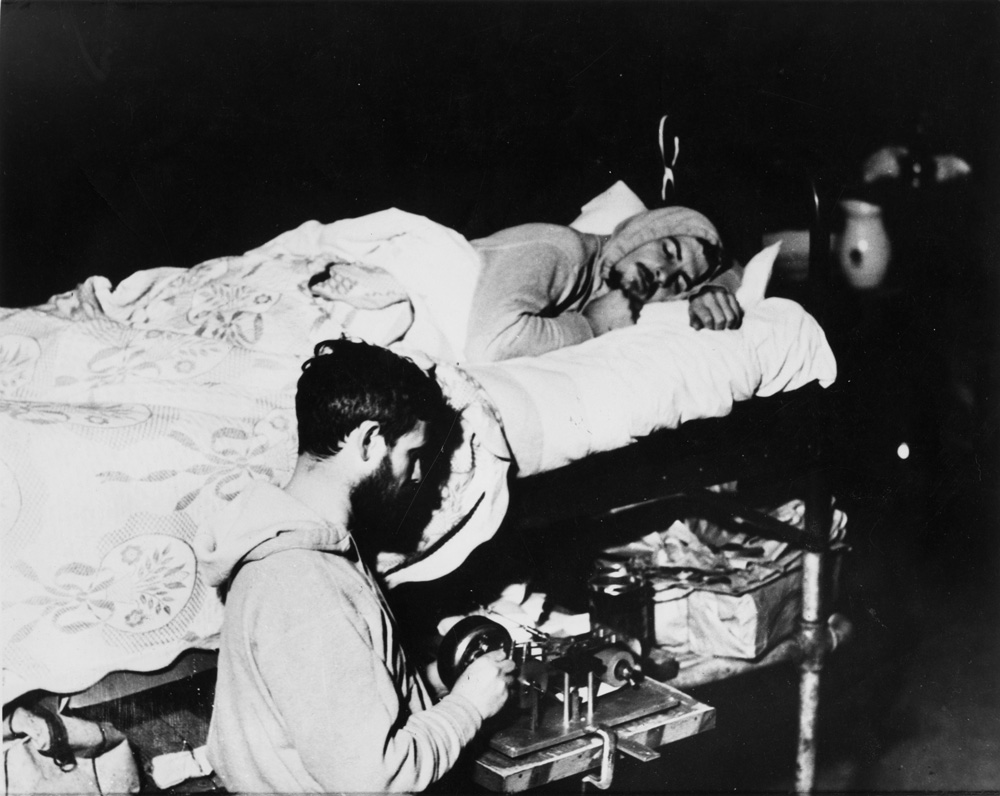
\includegraphics[width=0.5\textwidth]{Images/KleitmanCave}
	\caption{Nathaniel Kleitman (foreground), donning an impressive beard, measures the sleep of  Bruce Richardson \citep{universityofchicagophotographicarchiveKleitmanNathanielPhotographic}.}
	\label{Fig:Cave}
\end{figure}

Amazingly, it wasn't until 1938 that someone repeated this experiment on humans. Dr. Nathaniel Kleitman was a professor of of Physiology at University of Chicago who was later to discover Rapid-Eye Movement (REM) sleep; he is known as the father of sleep research. Together with his PhD student, Bruce Richardson, and a pair of metal beds, they descended into Mammoth Cave in Kentucky for 32 days without any natural lighting stimuli. They found that their sleep-wake cycle did not descend into sporadic bouts of sleep, but rather stayed at a periodic length of around 26 hours, undeniably longer than the 24 hour day. This showed that humans have an internal time-keeping system that lasts about (\textit{circa}) one day (\textit{dian}); they named it the circadian rhythm \citep{kleitmanSleepWakefulness1987}.

\citet{siffreTime1964} repeated this experiment, delving, himself, into a cavern for 2 months, and discovered much the same results. Meanwhile, \citet{vonaschoffSpontanperiodikMenschenBei1962} kept participants in a sealed cellar for 8-19 days, also discovering a circadian rhythm of over 25 hours.

As circadian rhythms are not 24 hours long, they need to be synchronised daily, and thus must rely on a periodic stimulus to entrain them. There were 5 factors that were thought could contribute to this entrainment of the circadian rhythm, as shown in Table \ref{Tab:Factors}.

\begin{table}
\caption{The 5 potential factors for circadian entrainment \citep{czeislerEntrainmentHumanOrcadian1981}}
\label{Tab:Factors}
\begin{tabular}{l l}
\hline
 & \textit{Factor} \\
\textbf{I.}& Knowledge of time of day \\
\textbf{II.}& Light Dark cycle \\
\textbf{III.}& Social Contacts \\
\textbf{IV.}& Timing of food availability \\
\textbf{V.}& Scheduling of bed rest and activity \\
\hline
\end{tabular}
\end{table}


It was originally thought that the light-dark (LD) cycle (Factor \textbf{I}) was too weak to entrain the circadian rhythms of humans, and that social cues (Factor \textbf{III}) were relied upon \citep{aschoffHumanCircadianRhythms1971}. 

Factor \textbf{I} (knowledge of time) was shown to be insignificant \citep{millsCircadianRhythmsThree1964}. Factor \textbf{II} (light-dark cycles) is the most powerful in many animals and plants, but \citet{aschoffHumanCircadianRhythms1971} concluded that this effect was too weak in humans, and that factor \textbf{III} (social cues) must be our central zeitgerber. However, when inspecting the facilities used for these experiments, \citet{czeislerEntrainmentHumanOrcadian1981} realised that the researchers ``\textit{permitted the subjects to use kitchen, bathroom, bedside and desk lamps as sources of self-selected light during the `dark' phase of each cycle}'', prompting a reassessment of the role of light in the entrainment of human circadian rhythms in which he found that light-dark cycles have a ``\textit{direct synchronising effect}'' on human circadian rhythms.

\subsection{Melatonin and Melanopsin}

The circadian rhythm is controlled by a part of the brain called the Hyperthalimus \citep{stephanCircadianRhythmsDrinking1972}. Specifically, in the Suprachiasmatic Nucleus (SCN), located above the optic nerve \citep{welshIndividualNeuronsDissociated1995}. The SCN sends signals to the pineal gland \citep{cassoneMelatoninRoleVertebrate1998, borjiginPINEALGLANDMELATONIN1999} which is responsible for the production and regulation of melatonin.\footnote{
There is much interest and mystery around the pineal gland, with many believing that it is where conciousness is generated in the brain \citep{bobMelatoninConsciousnessTraumatic2008}. Ren\'e Descartes referred to the pineal gland as the ``seat of the soul'' \citep{lokhorstDescartesPinealGland2020}.
}

Melatonin is known as the sleep hormone, or to some as the ``chemical expression of darkness'' \citep{reiterMelatoninChemicalExpression1991}, and builds up throughout the evening and is essential for sleep onset \citep{arendtImportanceRelevanceMelatonin2003}.

In 2000, a novel Opsin was found in the human eye \citep{provencioNovelHumanOpsin2000}. An opsin is a light-sensitive protein that exists in the visual cells in the eye and is what converts the energy from photons of light into electrical signals that are sent to the brain \citep{terakitaOpsins2005}. It was soon discovered that the action spectrum of this new opsin, malanopsin, did not match any of the action spectra of the known visual cells (rods and cones), implying there was a new cell that we were not yet aware of \citep{thapanActionSpectrumMelatonin2001}.\footnote{
Interestingly, melanopsiin has been found to be much more similar to invertebrate opsins than they are to visual mammalian opsins \citep{provencioMelanopsinOpsinMelanophores1998}. This, as well as the fact almost all animals produce melatonin, shows it is a truly ancient part of our biology \citep{daviesEvolutionFunctionMelanopsin2014}.
} 
This cell was found to be the intrinsically photosensitive Retinal Ganglion Cell (ipRGC) \citep{bersonPhototransductionRetinalGanglion2002}, the signals from which are what keeps the SCN entrained, but to not contribute to concious vision \citep{bersonPhototransductionGanglioncellPhotoreceptors2007}. This explains why some blind people have circadian rhythms that can be entrained with light, as discussed in the review by \citet{allenCircadianRhythmsBlind2019}.










\section{Health Implications}
\label{Sec:Health}


 in a meta analysis, \citet{sanchez-barceloClinicalUsesMelatonin2010} discusses the uses of melatonin in a host of situations, including ``ocular diseases, blood diseases, gastrointestinal tract diseases, cardiovascular diseases, diabetes, rheumatoid arthritis, fibromyalgia, chronic fatigue syndrome, infectious diseases, neurological diseases, sleep disturbances, aging and depression [as well as being] used as a complementary treatment in anaesthesia, hemodialysis, in vitro fertilization and neonatal care''




%Once the morning comes, the cortisol awakening response (CAR) is triggered, flooding the body with cortisol, the hormone of wakefulness and alertness \citep{friesCortisolAwakeningResponse2009}.
%



% The SCN, in turn, signals to the pineal gland to stop producing melatonin \citep{lewyLightSuppressesMelatonin1980, owenMelatoninSuppressionHuman1992, gooleyExposureRoomLight2011}.
%
%Even light as dim as ~50 Lux can affect serum melatonin levels \citep{laaksoOnehourExposureModerate1993, 
%zeitzerSensitivityHumanCircadian2000}.
%
%




